\section{Software PWM}
\label{sec:swpwm}

The motor used to position the arm in this project is driven by a MOSFET H-bridge.
For greatest efficiency, MOSFETS should always be switched to their on or off state. 
The on-off switching performed by the MOSFETs, can used to generate a power signal with a controllable average value using pulse width modulation (PWM).
The PWM for this project was designed to operate in the range of 9.5V to -9.5V and was implemented in Matlab’s Simulink environment after it was determined that accurate control couldn’t be achieved using the external op-amp oscillator, peak detector and additional circuitry.
A Simulink block diagram showing the PWM implementation may be seen in Figure \ref{fig:SWPWM}.

The key component in this diagram is the \q{PWM Source}, a repeating ramp from zero to one which resets every 10 ms.
As such, the nominal PWM frequency is 100 Hz.
Given the controller sampling rate of $200 \mu s$ and output range of 0-9.5 Volts for each side %Not really clear
of the PWM generator, a control resolution of approximately 190 mV is achieved.
When compared to the very fine resolution and approximate 300 Hz frequency of the op-amp based oscillator and peak detector, the software PWM appears to be a poor choice.
It is however vastly more deterministic and far less prone to external distrubances.
An important consideration, due to the bound on sampling rate, when choosing the PWM frequency is the tradeoff between resolution and frequency. 
By increasing the switching frequency, the PWM resolution will be directly reduced.

Ideally, the PWM should have a switch frequency much higher than the dynamics of the system, motor and controller, such that the motor appears to be powered by a true DC voltage source.
The PWM frequency should be much greater than the natural frequency of the system to prevent interference and phase delay. 
Equivalently stated, the input signal to the PWM generator should be stable within the period of each pulse.
This desire for separation between the PWM frequency and system natural frequency is antithetical to the desire for increased natural frequency to improve system response and reduce settling time.
Conversely, there is also a desire for greater PWM resolution such that the motor can be positioned accurately.
Increasing resolution also helps to prevent undesirable limit-cycling; a source of inaccuracy and mechanical vibration.

%TODO: Some sort of conclusion or something?

%At low frequencies, this switching waveform may have a lot of spikes associated with it.
%This characteristic is undesirable as it will cause significant power loss in the resistances of the wires, MOSFETs, and motor windings.
%Also, if the supply voltage isn't switched fast enough, there will be time for the speed to change and hence the speed won't be steady.
%With higher the switching frequency, a more stable current waveform in the motor is achieved since the inductance of the motor will smooth this out to an average DC current level proportional to the PWM demand.
%Increasing frequency has to be balanced by the fact that the PWM's resolution is dependent on the switching frequency.

%Undesirable limit-cycling occurs in a low resolution PWM signal such that switching is quantized and limited to only at certain points in time.

\begin{figure}[h]
    \centering
    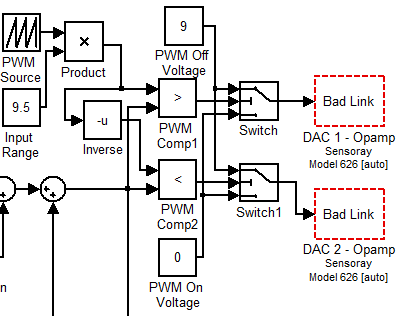
\includegraphics[scale=0.75]{images/SWPWM.PNG}
    \caption{Software PWM Simulink Schematic}
    \label{fig:SWPWM}
\end{figure}
